\section{What this means for assignment practice}\label{sec:practice}

This section translates the results into the terms of a modeller who runs assignments at increasing demand and watches total travel time or the price of anarchy. Unless stated otherwise, the numbers are high-precision numerical computations (50--60 significant digits) for the five-link example, made with the physical costs. They agree with the exact series.

\subsection{Hidden activation below assignment tolerance}

Table~\ref{tab:hidden} shows how little the new route is used after the expansion at $t=1$.

\begin{table}[htbp]
\centering\small
\begin{tabular}{rrrr}
\toprule
$\delta=t-1$ & connector flow $x$ & $x$ as \% of A's demand & $(E-E_0)/E_0$\\
\midrule
$0.01$ & $6.33\times10^{-7}$ & $1.6\times10^{-5}$ & $-4.9\times10^{-12}$\\
$0.05$ & $6.31\times10^{-5}$ & $1.5\times10^{-3}$ & $-1.0\times10^{-8}$\\
$0.10$ & $3.88\times10^{-4}$ & $8.8\times10^{-3}$ & $-2.0\times10^{-7}$\\
$0.20$ & $1.93\times10^{-3}$ & $4.0\times10^{-2}$ & $-2.7\times10^{-6}$\\
\bottomrule
\end{tabular}
\caption{The five-link example after its expansion. Total cost $E$ is compared with the cost $E_0$ of the same network without the connector. \status{numerical}}
\label{tab:hidden}
\end{table}

Ten per cent more demand moves about $0.01\%$ of commodity A onto the new route and changes total cost by about two parts in ten million. Typical assignment runs stop at relative gaps between $10^{-4}$ and $10^{-6}$. The connector carries less than $10^{-4}$ of A's demand up to $\delta\approx0.105$, less than $10^{-5}$ up to $\delta\approx0.043$, and less than $10^{-6}$ up to $\delta\approx0.019$. The relative change in total cost stays below $10^{-5}$ up to $\delta\approx0.31$ and below $10^{-6}$ up to $\delta\approx0.15$. An assignment at ordinary tolerance would therefore classify the connector as unused over a wide demand range, and the total-cost curve would show no trace of the change.

\subsection{Link flows reveal the change earlier than totals}

The transition is not equally hidden in all quantities. The connector flow and every bank load differ from their no-connector continuations at order $\delta^3$, so link flows are $C^2$ but not $C^3$. The commodity costs differ by $\mp\frac{168}{625}\delta^3$ (A gains, B loses), and are also only $C^2$. Only the aggregates $E$ and $P$ hide two further orders, through the cancellation \eqref{eq:Ecancel}. So link-level and commodity-level monitoring is more sensitive than monitoring total travel time or the price of anarchy. The contact order is also measurable: it is the slope of $\log|\Delta|$ against $\log|t-t_0|$, which can be estimated from assignments at a few demand levels.

\subsection{Near-matches leave tiny kinks}

Exact equality of slopes is exceptional at nondegenerate breakpoints (Theorem~\ref{thm:generic}). Near-equality is not, because the restored kink is small (Proposition~\ref{prop:perturbation}). If the connector's free-flow time is $1\%$ too high ($\varepsilon=+0.01$), the expansion moves to $t\approx1.330$ and the slope of $E$ drops there by $0.0039$, which is about $0.012\%$ of $E'(1)=32.8$. If it is $1\%$ too low ($\varepsilon=-0.01$), the expansion moves to $t\approx0.787$ and the drop is $0.079$, about $0.24\%$. At $\varepsilon=+0.1$ the drop is $0.028$, under $0.1\%$. The asymptotic law in \eqref{eq:exactperturbation} is accurate only for much smaller $|\varepsilon|$, so these values come from the exact formula, checked by finite differences. For $\varepsilon\le-0.056$ there is no expansion near $t=1$ at all, because the gap on $[0.58,1]$ never falls below $-0.0557$. \status{numerical}

\subsection{No Braess effect at onset; the optimum moves first}

At the expansion the new route lowers total cost relative to the network without it: $E-E_0=-k_E\delta^5<0$. This is the opposite of Braess's paradox \cite{Braess1968,SteinbergZangwill1983}, though only by a tiny amount. In the bank-swapped contraction the connector is used below $t=1$, and there $E-E_0=+k_E|\delta|^5>0$: using the connector raises total cost slightly, a weak Braess-type effect. The system optimum already uses the connector at $t=1$, with optimal connector load $0.00643$. Here $S(1)=19.762875963175$, both by direct optimisation and by the scaling formula, and $P(1)\approx1.0120$. The jump of $P^{(5)}$ at $t=1$ is about $-6.58$. By Theorem~\ref{thm:optimumtransition}, the optimum's own transition at $t=1/\gamma\approx0.669$ is a second hidden transition of $P$, with $P\in C^5\setminus C^6$ there.

Two caveats concern the example itself. First, it has further breakpoints at low demand: the connector is also used for $t\in(0.2105,0.5839)$, and bank edge $G_3$ is unused below $t\approx0.631$. The statements above are local to $t=1$ and to $t=1/\gamma$. Second, every result here concerns deterministic user equilibrium. Under logit stochastic user equilibrium every route carries flow, there are no breakpoints, and the question does not arise.

\subsection{An exploratory test on Sioux Falls}\label{sec:sioux}

To see whether calibrated networks show anything similar, we solved the deterministic user equilibrium of the Sioux Falls test network \cite{LeBlanc1975,TNTP} (24 nodes, 76 links, BPR exponent~4) for demand multipliers $\theta\in[0.05,1.5]$. A path-based solver reached relative gap $10^{-12}$ at every point. \status{exploratory}

\begin{itemize}[nosep]
\item On $\theta\in[0.5,1.5]$ every link carries flow, so there is no link-level activation near nominal demand. We did not analyse route-level changes, which path-flow nonuniqueness makes delicate.
\item The only link activations are the two directions of one corridor, link $17\to10$ at $\theta^*\approx0.25916$ and link $10\to17$ at $\theta^*\approx0.26021$.
\item Both activations are transverse. The new link's flow grows linearly, with log--log slope $1.0000\pm2\times10^{-4}$ for $\theta-\theta^*\in[10^{-5},3\times10^{-3}]$, and the slope of total travel time drops by about $3.4\%$ and $3.3\%$.
\item Even so, solvers stopped at relative gaps of $10^{-4}$ or $10^{-5}$ (Frank--Wolfe, and the same path-based method stopped early) report the link as used already before $\theta^*$. Their link-flow errors of tens of vehicles exceed the true new flow within about $10^{-3}$ of $\theta^*$.
\end{itemize}

This one network agrees with Theorem~\ref{thm:generic}: its activations are transverse and produce visible kinks. It also shows the practical point of Section~\ref{sec:practice} in milder form. At ordinary tolerances, the link-usage pattern near an activation is unreliable even when the kink is clear. The illustration covers one test network and one artificial demand path, and it says nothing about how often near-tangent activations occur. Wang, Shao and Wu \cite{WSW2026} also use Sioux Falls to illustrate demand dependence of the price of anarchy.

\begin{figure}[htbp]
\centering
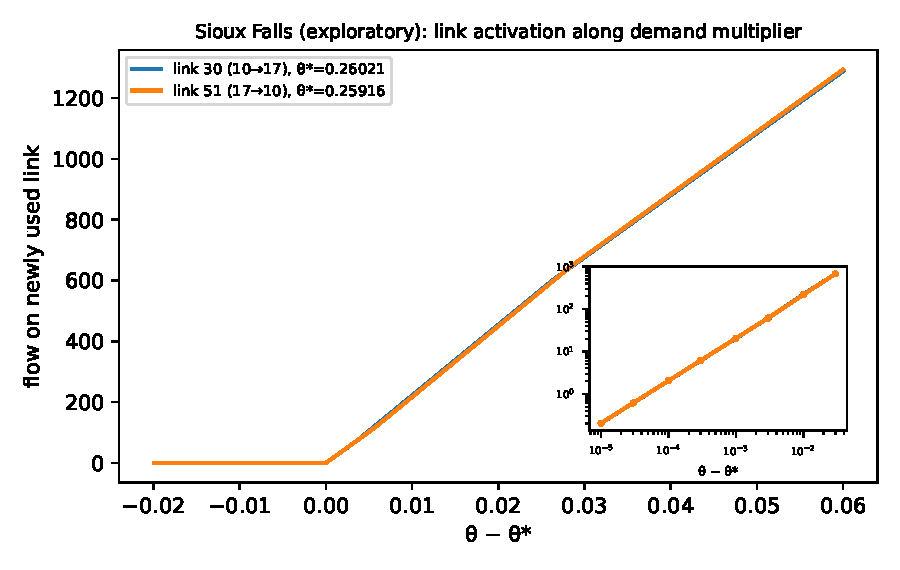
\includegraphics[width=0.78\linewidth]{../figures/sioux_falls.pdf}
\caption{Sioux Falls: flow on a newly used link against $\theta-\theta^*$, with a log--log inset showing linear growth. \status{exploratory}}
\label{fig:sioux}
\end{figure}
